\documentclass[a4paper,11pt]{report}
\usepackage[french]{babel}
\usepackage[T1]{fontenc}
\usepackage[utf8]{inputenc}
\usepackage{lmodern}
\usepackage{microtype}
\usepackage{hyperref}
\usepackage{tabulary}
\usepackage{framed}
\usepackage{fancyhdr}
\usepackage{amsmath}
\usepackage{bbm}
\usepackage{graphicx}
%\usepackage{pst-all}
%\usepackage{xcolor}
%\usepackage{nopageno}

%\newcommand{\latin}[1]{\textit{#1}}

\usepackage[margin=1.0in]{geometry}

%%%%%%%%%%%%%%
%\usepackage{geometry}
 %\geometry{
% a4paper,
 %total={210mm,297mm},
 %left=20mm,
 %right=20mm,
 %top=20mm,
 %bottom=20mm,
 %}
 %%%%%%%%%%%%%%
 
\pagestyle{empty}

\pagestyle{fancy}
\fancyhead{}
\renewcommand{\headrulewidth}{0.5pt}
\fancyhead[R]{\textit{\nouppercase{\rightmark}}}
\fancyfoot{}
\renewcommand{\footrulewidth}{0.5pt}
\fancyfoot[L]{\textit{\nouppercase{\leftmark}}}
\fancyfoot[R]{\thepage}
  
\begin{document}
	\begin{titlepage}
		\vspace*{\stretch{2}}
		\begin{center}
			\large\bfseries\itshape Stage ETE 2015\\
		\end{center}
		\noindent\rule{\linewidth}{3pt}

		\begin{center}
			\Huge\bfseries\itshape Description du système\\
		\end{center}
		
		\noindent\rule{\linewidth}{3pt}
		\begin{center}
			\bfseries
			\large F-PHT \\
			\large Un système d'index de filtres de Bloom pour la recherche d'information par mots clés
		\end{center}
		\vspace*{\stretch{2}}
		\begin{center}
			Réalisé par \textbf{DOAN} Cao Sang \\
			Encadrant: M. \textbf{MAKPANGOU} Mesaac, Regal
		\end{center}
		\vspace*{\stretch{0.5}}
		\begin{center}
			1 Juillet 2015
		\end{center}
	\end{titlepage}

\tableofcontents

\chapter{Vue globale}
\section{Prefix Hash Tree (PHT)}
	Un arbre préfixe est un arbre numérique ordonné qui est utilisé pour stocker une table associative où les clés sont généralement des chaînes de caractères. Contrairement à un arbre binaire de recherche, aucun nœud dans le trie ne stocke la chaîne à laquelle il est associé. C'est la position du nœud dans l'arbre qui détermine la chaîne correspondante\footnote{Wikipédia}.
	
	Pour tout nœud, ses descendants ont en commun le même préfixe. La racine est associée à la chaîne vide. Des valeurs ne sont pas attribuées à chaque nœud, mais uniquement aux feuilles et à certains nœuds internes se trouvant à une position qui désigne l'intégralité d'une chaîne correspondante à une clé.
	
	Pour faire une recherche d'une valeur associée à une clé, au départ, on se situe à la racine de l'arbre, en prenant le premier élément de la clé de la requête, on trouve le chemin étiqueté par cet élément, s'il n'existe pas, on est sûr que cette clé n'est pas dans l'arbre. Dès que l'on trouve le chemin, on arrive sur le bon nœud et continue en prenant le deuxième élément de la clé de requête, on applique cette méthode jusqu'à quand on trouve cette clé et se termine sur une feuille.
	
	\begin{figure}[!htbp]
	\centering
	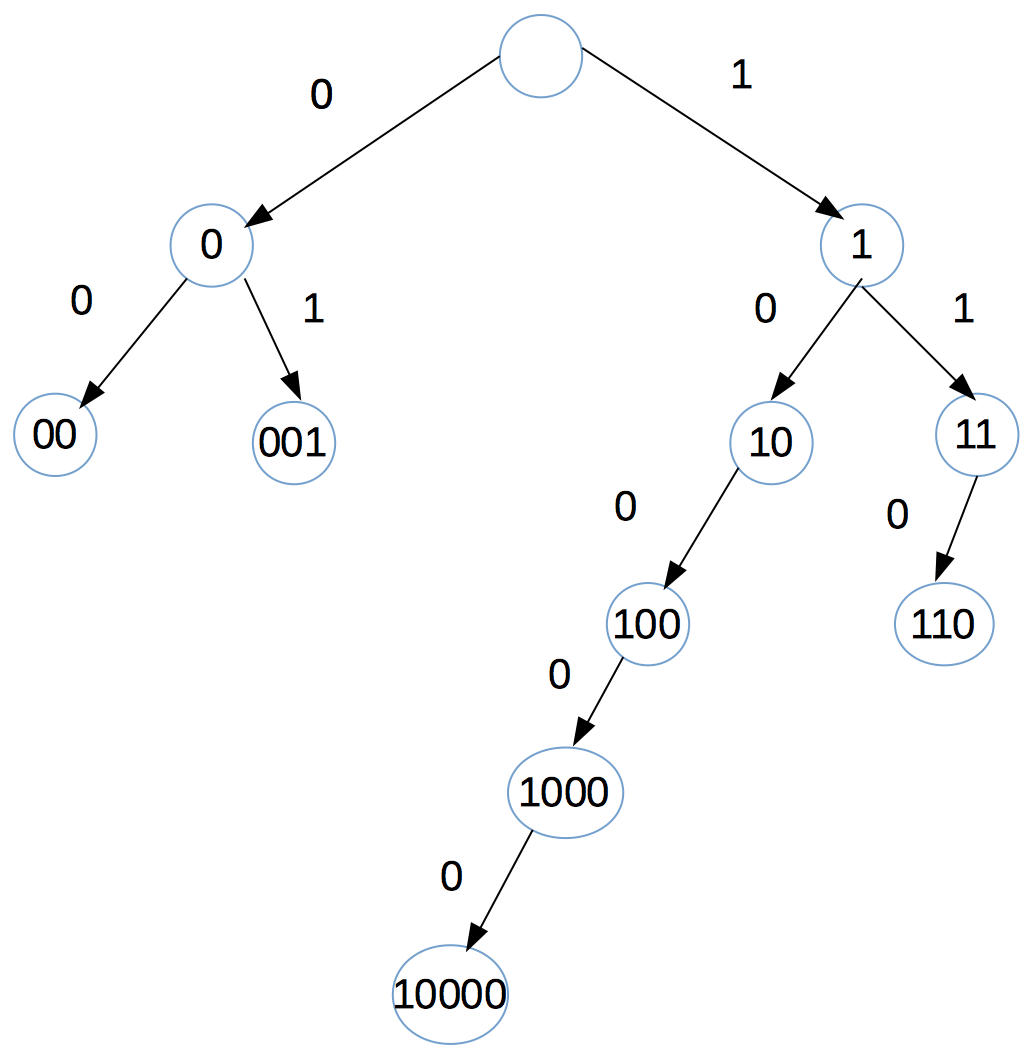
\includegraphics[width=12cm]{PHT.eps}
	\caption{Arbre de préfixe}
	\label{PHT}
	\end{figure}	

\newpage	
	
\section{F-PHT}
	F-PHT est un arbre préfixe de "multibit". Pour stocker une clé, on suit le chemin étiqueté par les fragments successifs de cette clé (dans l'ordre de leur rang) jusqu'à ce qu'on arrive sur une feuille pouvant stocker cette clé.

	Un fragment est un morceau d'une clé (sous-ensemble de bits). Si on considère les clés de taille \textit{m}, le système découpe chaque clé en \textit{f} fragments de taille identique. Par convention, ces fragments sont numérotés de \textit{0} à \textit{f-1}.
	
	\begin{table}[!h]
		\centering		
		\begin{tabular}{|l|*{14}{c|}r|}
		\multicolumn{1}{c}{{\scriptsize 15}} &\multicolumn{1}{c}{}&\multicolumn{1}{c}{}&\multicolumn{1}{c}{}&
		\multicolumn{1}{c}{}&\multicolumn{1}{c}{}&\multicolumn{1}{c}{}&\multicolumn{1}{c}{}&
		\multicolumn{1}{c}{}&\multicolumn{1}{c}{}&\multicolumn{1}{c}{}&\multicolumn{1}{c}{}&
		\multicolumn{1}{c}{}&\multicolumn{1}{c}{}&\multicolumn{1}{c}{}&\multicolumn{1}{c}{{\scriptsize 0}}\\
		\hline
			1 & 0 & 0 & \multicolumn{1}{c||}{0} & 
			1 & 1 & 0 & \multicolumn{1}{c||}{1} & 
			0 & 0 & 0 & \multicolumn{1}{c||}{0} & 
			1 & 0 & 1 & 0 \\
		\hline
		\end{tabular}
		\caption{Exemple le filtre de Bloom}
		\label{fragment/filtredeBloom}
	\end{table}
	
	La table \ref{fragment/filtredeBloom} représente une clé de taille \textit{m = 16} bits, elle est ensuite découpée en \textit{f = 4} fragments. Le premier fragment est la suite de bits \textit{"1000"} qui se trouve les plus à gauche de cette clé. Le dernier est \textit{"1010"}.
	
	\begin{figure}[!htbp]
	\centering
	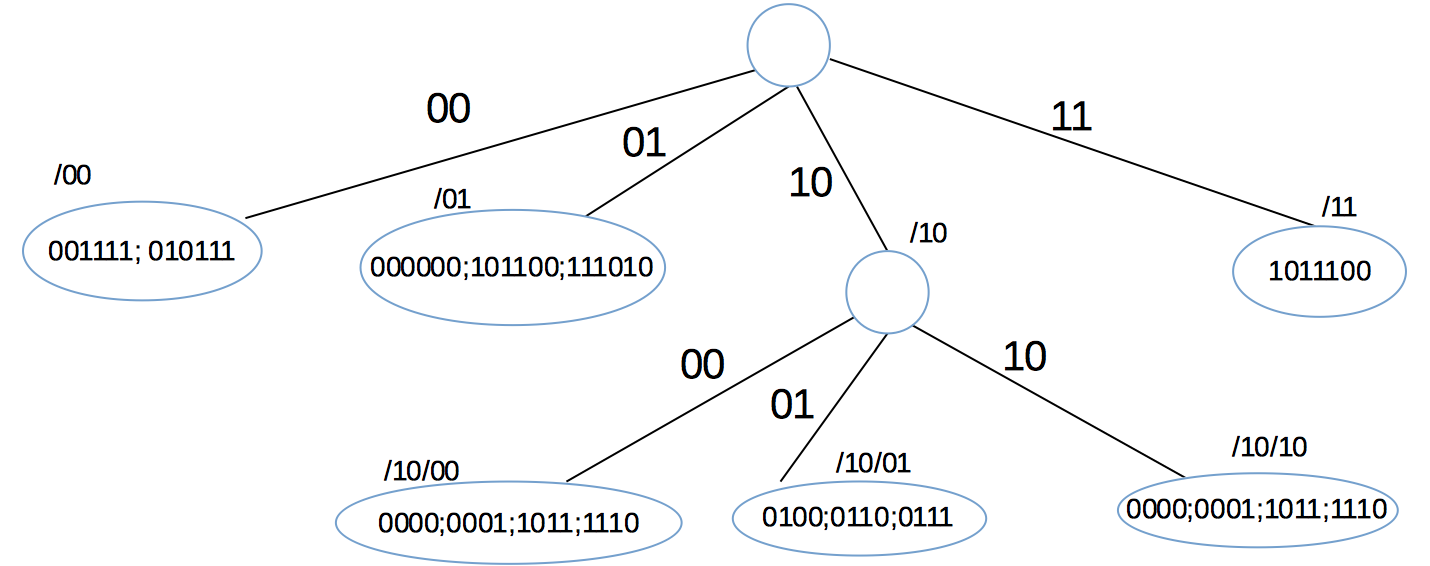
\includegraphics[scale=0.70]{F-PHT_2.eps}
	\caption{Arbre F-PHT}
	\label{F-PHT2}
	\end{figure}	
	
	La figure \ref{F-PHT2} représente l'arbre F-PHT qui stocke une clé de taille \textit{m = 8} bits, la taille d'un fragment est de 2 bits. Au dessus de chaque nœud (interne ou feuille) se trouve son identifiant unique et il caractérise également le chemin unique conduit vers ce nœud.
	
\chapter{Système d'indexation}
\section{Objectif}
	Les clés indexées sont des filtres de Bloom de taille \textit{m}.
	L'objectif du système est d'une part de stocker les filtres de Bloom donnés par les utilisateurs, d'autre part de permettre de rechercher tous les filtres de Bloom (stockés dans le système) qui sont sur-ensemble d'un filtre de Bloom caractérisant des mots clés d'une requête.

\section{Architecture d'un système d'indexation}
	Le système d'indexation est sur un ensemble de serveurs d'index répartis sur plusieurs machines. Chaque serveurs gère un ou plusieurs nœuds de ce système.

\section{API du système d'indexation}
	
	
\chapter{Fonctionnement du système}
\section{Données de chaque nœud dans l'arbre}
\section{Protocole}

	Ce protocole porte des actions entre le client et le système comme : add, search, remove.
	
	Lors que le système reçoit un filtre de Bloom à indexer, il appelle simplement cette méthode \textbf{add}. Cette méthode envoie un message d'ajout à la racine. Ensuite, la racine route ce message jusqu'à la feuille qui s'occupe ce filtre grâce à la valeur de fragment de rang \textit{i}.

\subsection{Cas d'un nœud feuille}
	Lors qu'une feuille reçoit la demande \textbf{add} d'un filtre de Bloom, elle cherche l'indice où le met dans la table \textit{LocalRoute}. Si l'entrée est pleine, pour chaque entrée de la table, elle demande le système de créer un nœud correspondant, et ajoute son identifiant dans la nouvelle table \textit{LocalRoute}. Cette nouvelle table remplace l'autre après les transferts des données vers les fils convenables. Si l'entrée est libre, la feuille ajoute simplement. Elle devient un nœud.
	
\subsection{Cas d'un nœud}
	Un nœud reçoit la demande d'ajout d'un filtre de Bloom est simple, en regardant dans sa table \textit{LocalRoute}, trouve une entrée qui satisfait la requête et la route vers ce fils.
	
\section{Recherche des filtres de Bloom}
	Cette commande \textbf{search} est aussi envoyée vers la racine, par contre, elle renvoie cette requête vers tous les fils qui contient.
	
\subsection{Cas d'un nœud feuille}
	Une feuille reçoit la requête, elle compare la requête avec les filtres dans sa table \textit{LocalRoute}, et collecte tous les filtres qui contiennent la requête. Une fois, tous les filtres satisfaisants sont renvoyés vers la racine.

\subsection{Cas d'un nœud}
	Un nœud compare aussi la requête avec les entrées dans \textit{LocalRoute}, toutes les entrées qui contiennent la requête sont sélectionnées pour récupérer tous les nœuds afin de leur renvoyer la requête.
	
\section{Suppression d'un filtre de Bloom}
	Cette action \textbf{remove} fonctionne exactement comme l'ajout d'un filtre de Bloom, la racine route la requête de suppression vers le fils qui gère cette requête. Dès qu'elle arrive à la feuille, cette feuille cherche dans sa propre table \textit{LocalRoute} une entrée correspondante et la supprime. Si cette table devient vide après la suppression, elle demande de la supprimer au système, en plus, le système se charge de notifier son père la disparition de son fils pour qu'il puisse supprimer l'entrée de son fils dans sa table de routage \textit{LocalRoute}. Du coup, si sa propre table \textit{LocalRoute} devient vide après la suppression de son fils, il aussi demande de se supprimer au système et notifie son père. Ces opérations continuent jusqu'à quand il n'y a plus de table \textit{LocalRoute} vide.

\end{document}









